%\linenumbers*
\chapter{EFFECT OF IN-STORM RAINFALL INTENSITY CHANGES ON SOIL EROSION}
\label{sec:EFFECTSOFRAINFALLINTENSITYCHANGESONSOILEROSION}

\section{Introduction}
\label{sec:IntensiyPatternsIntroduction}
This chapter investigates the effect of rainfall intensity changes within
storm duration. WSIP (Within-Storm Intensity Pattern) means the temporal shape
of the storm's WSIV (Within-Storm Intensity Variation). It could be increasing,
decreasing or constant, or more complex. This is also related to the
time-to-peak parameter in WEPP.

\section{Simulation Data and Methods}
\label{sec:IntensiyPatternsMethods}

% In the previous investigation, it was assumed that rainfall intensity was
% constant during a storm period. In reality, rainfall intensity is constantly
% changing throughout the storm period. This will certainly have an effect on soil
% erosion.

A design storm was used. Rainfall intensity of the storm varied
to increasing, decreasing, increasing-decreasing and constant while keeping the
amount of rainfall unchanged.
%Intensity varied rainfall data (actually WEPP disaggregated data because of
%EUROSEM)
Only one peak intensity per storm was assumed for model simulations.

Two designed storms with average intensity of 10mm/hr (120 mm for 12 hrs)
and 60 mm/hr (120 mm for 2 hrs) were used for WEPP and EUROSEM simulations.
A designed storm with average rainfall intensity of 120 mm/hr was used for
RillGrow simulation.

The effects of these intensity changes on runoff and soil loss rate were
investigated using three models---WEPP, EUROSEM and RillGrow.
WEPP, EUROSEM and RillGrow are used to simulate runoff and soil loss, and
the effects of patterns were compared.

\begin{figure}[htbp]
  \centering
  \subfloat[]{%
  \label{fig:weppinputincrease2hr}
  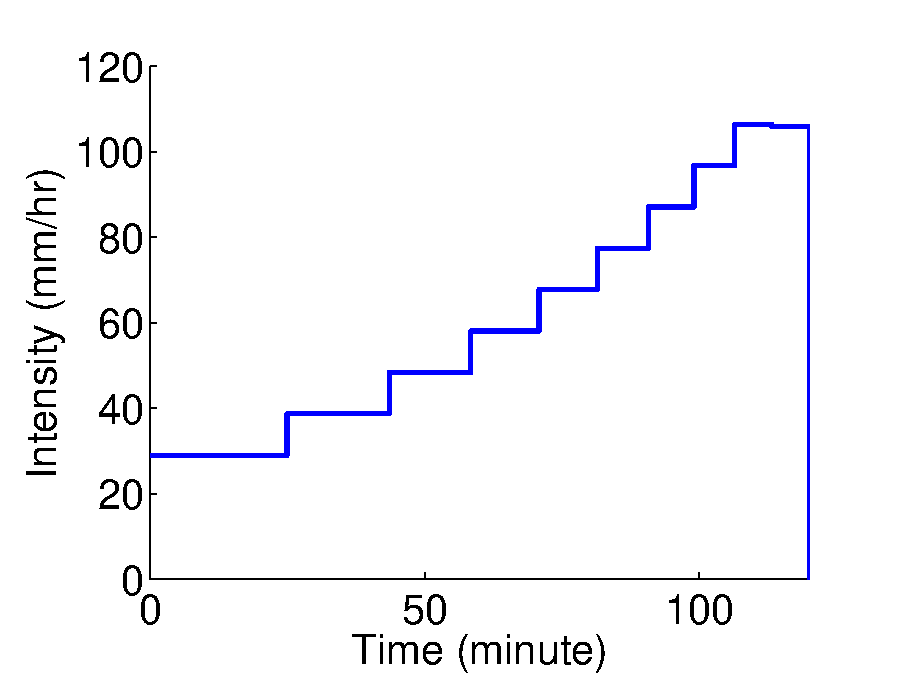
\includegraphics[width=0.24\textwidth]{./img/wepp_input_increase_2hr}}
  \subfloat[]{%
  \label{fig:weppinputdecrease2hr}
  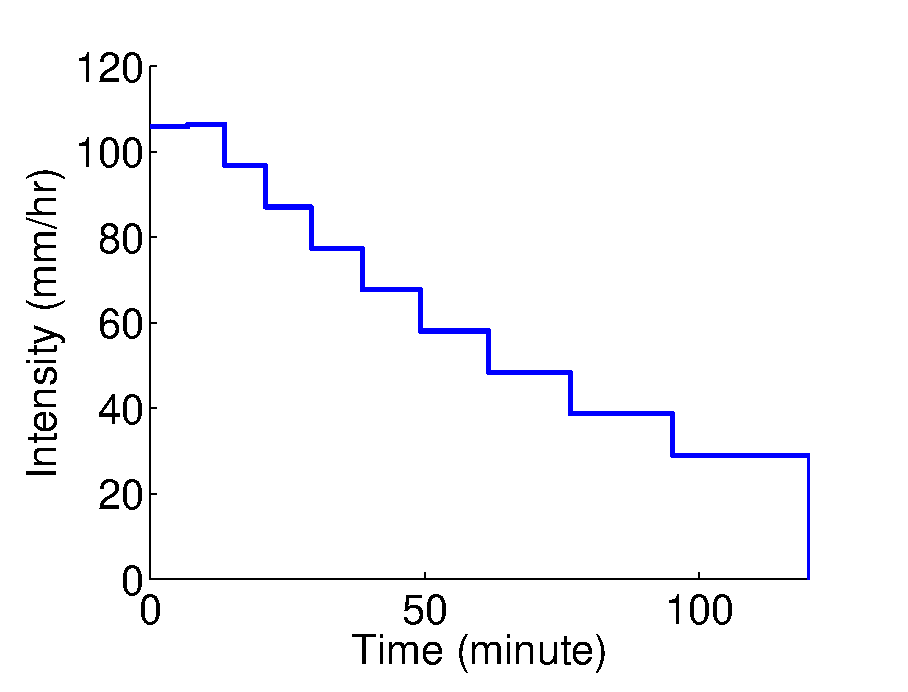
\includegraphics[width=0.24\textwidth]{./img/wepp_input_decrease_2hr}}
  \subfloat[]{%
  \label{fig:weppinputcontrol2hr}
  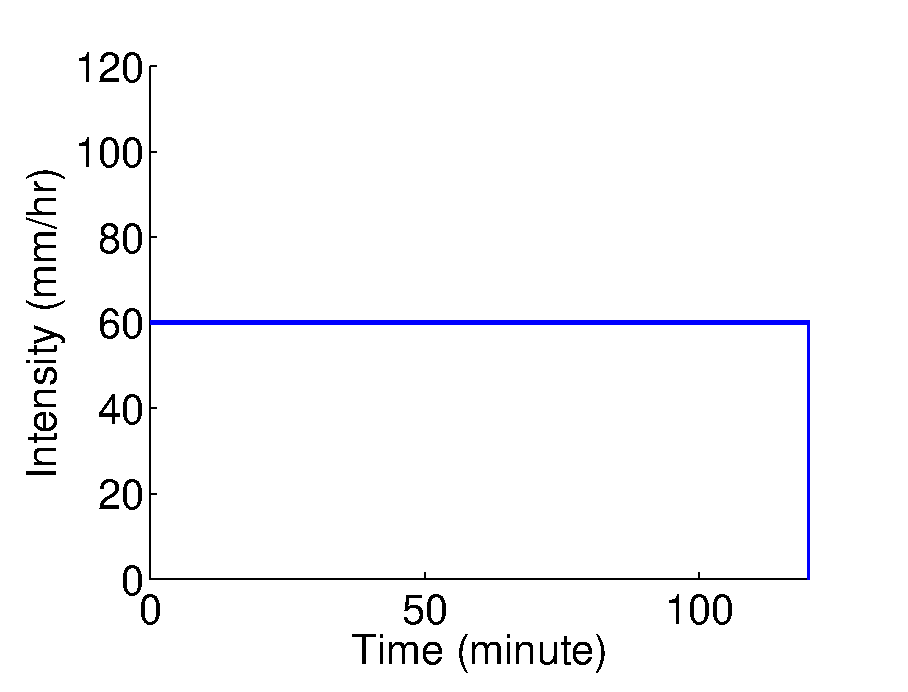
\includegraphics[width=0.24\textwidth]{./img/wepp_input_constant_2hr}}
  \subfloat[]{%
  \label{fig:weppinputincreasedecrease2hr}
  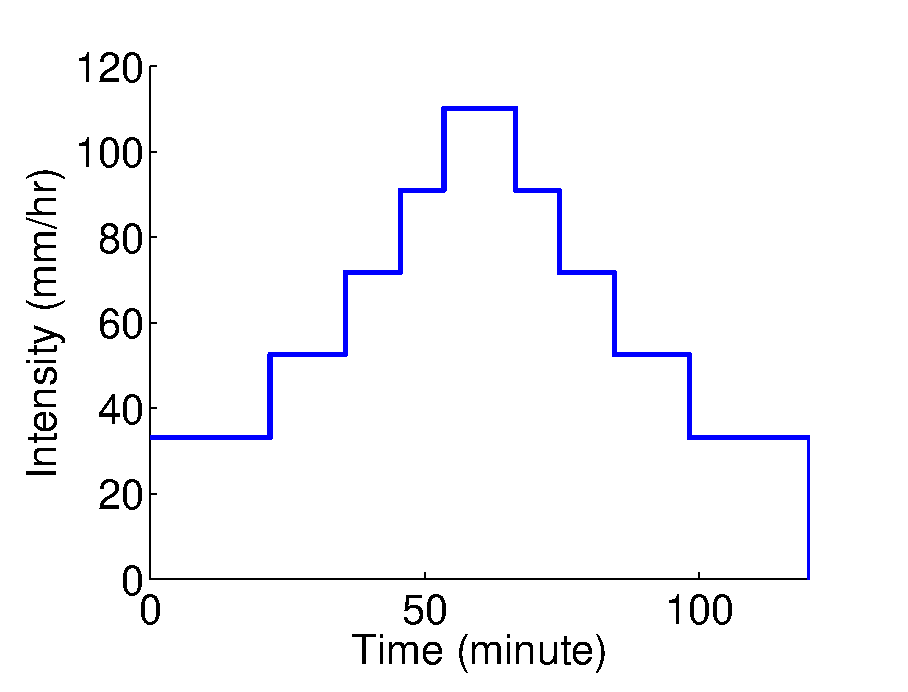
\includegraphics[width=0.24\textwidth]
{./img/wepp_input_increase_decrease_2hr}}
  \caption[Intensity patterns of a convective storm for WEPP and EUROSEM
simulations.]{Intensity patterns of a convective storm for WEPP and EUROSEM
simulations. All the inputs have the same total rainfall amount (120 mm) and
duration (2 hour). Note the scales of the axes.}
  \label{fig:weppeurosemintensityinputstwohours}
\end{figure}

\begin{figure}[htbp]
  \centering
  \subfloat[]{%
  \label{fig:weppinputincrease6hr}
  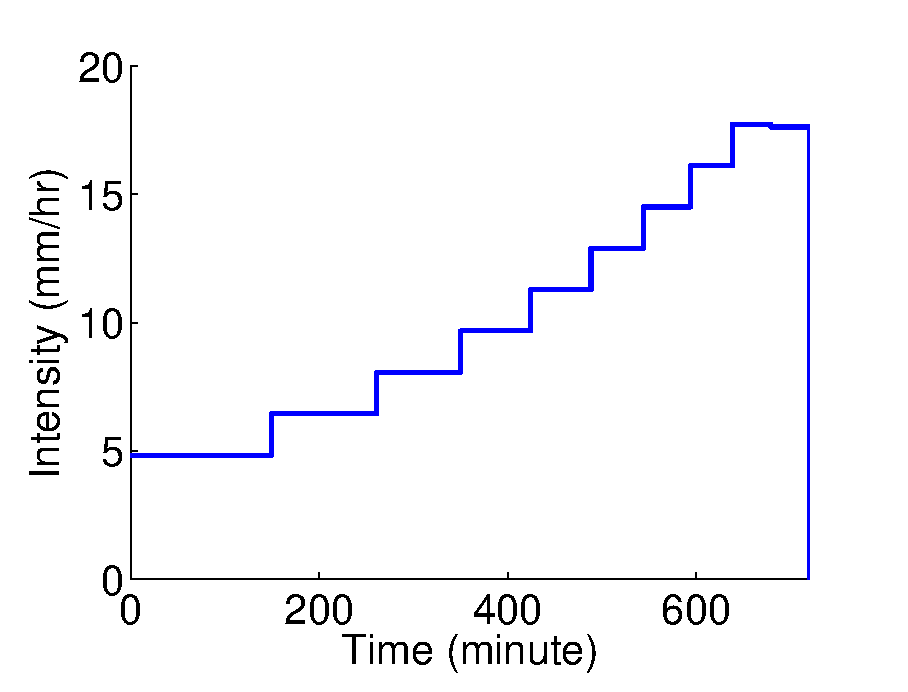
\includegraphics[width=0.24\textwidth]{./img/wepp_input_increase_6hr}}
  \subfloat[]{%
  \label{fig:weppinputdecrease6hr}
  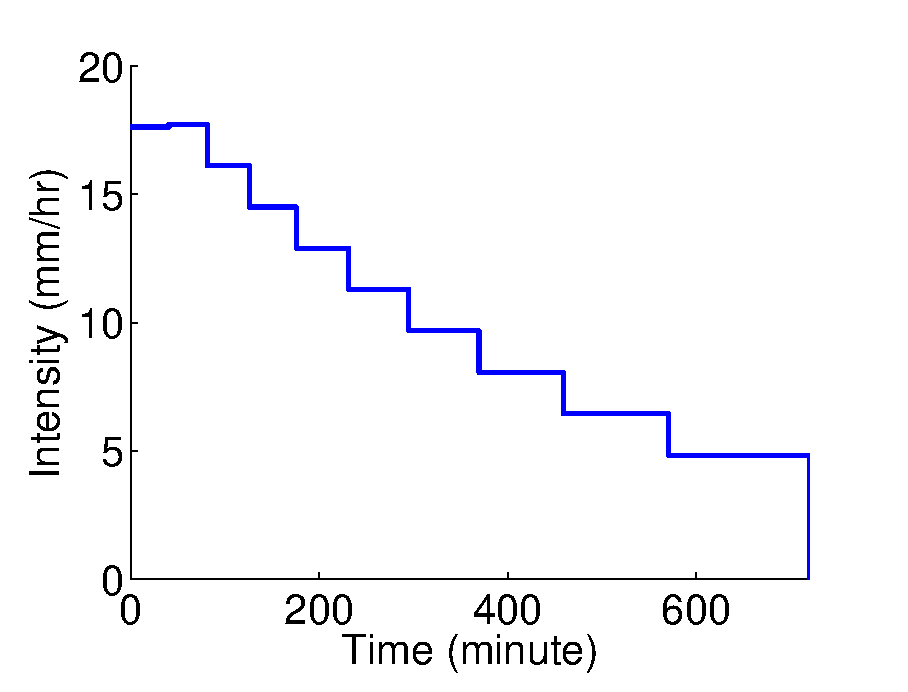
\includegraphics[width=0.24\textwidth]{./img/wepp_input_decrease_6hr}}
  \subfloat[]{%
  \label{fig:weppinputcontrol6hr}
  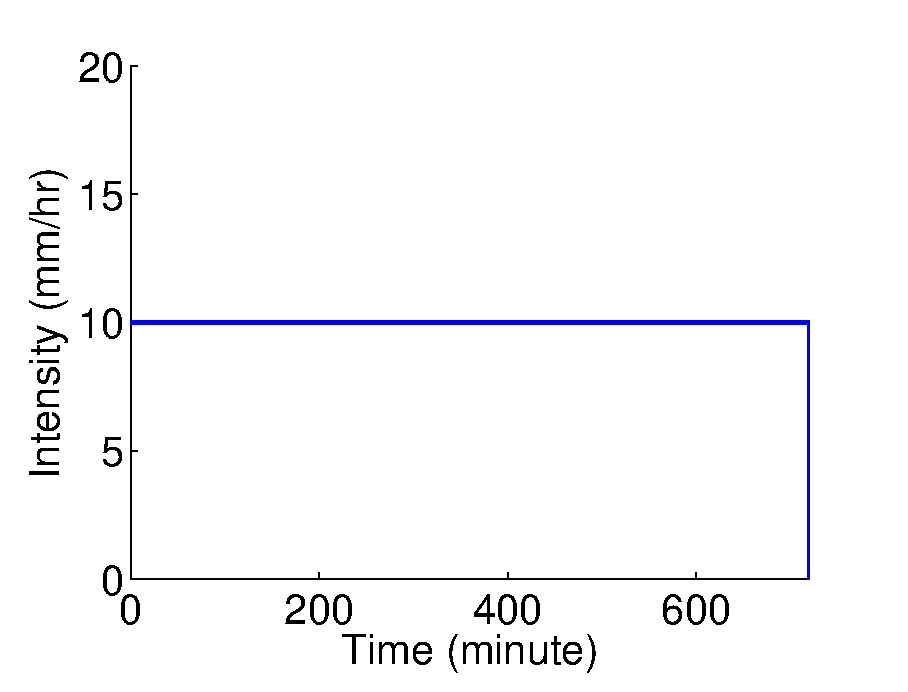
\includegraphics[width=0.24\textwidth]{./img/wepp_input_constant_6hr}}
  \subfloat[]{%
  \label{fig:weppinputincreasedecrease6hr}
  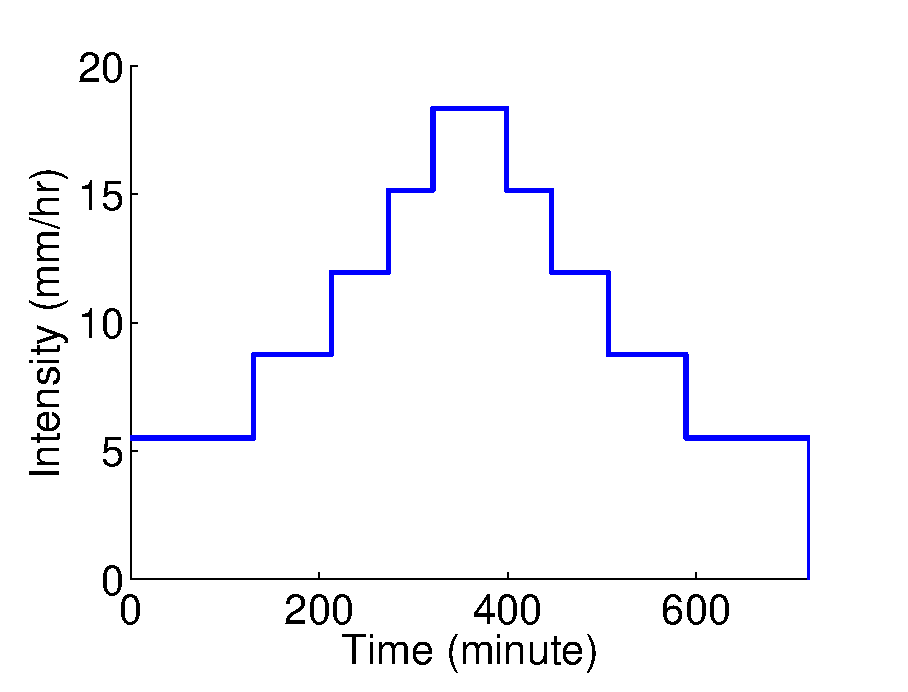
\includegraphics[width=0.24\textwidth]
{./img/wepp_input_increase_decrease_6hr}}
  \caption[Intensity patterns of a stratiform storm for WEPP and EUROSEM
simulations.]{Intensity patterns of a stratiform storm for WEPP and EUROSEM
simulations. All the inputs have the same total rainfall amount (120 mm) and
duration (12 hour). Note the scales of the axes.}
  \label{fig:weppeurosemintensityinputssixhours}
\end{figure}


\begin{figure}[htbp]
  \centering
  \subfloat[]{%
  \label{fig:rg2inputincrease}
  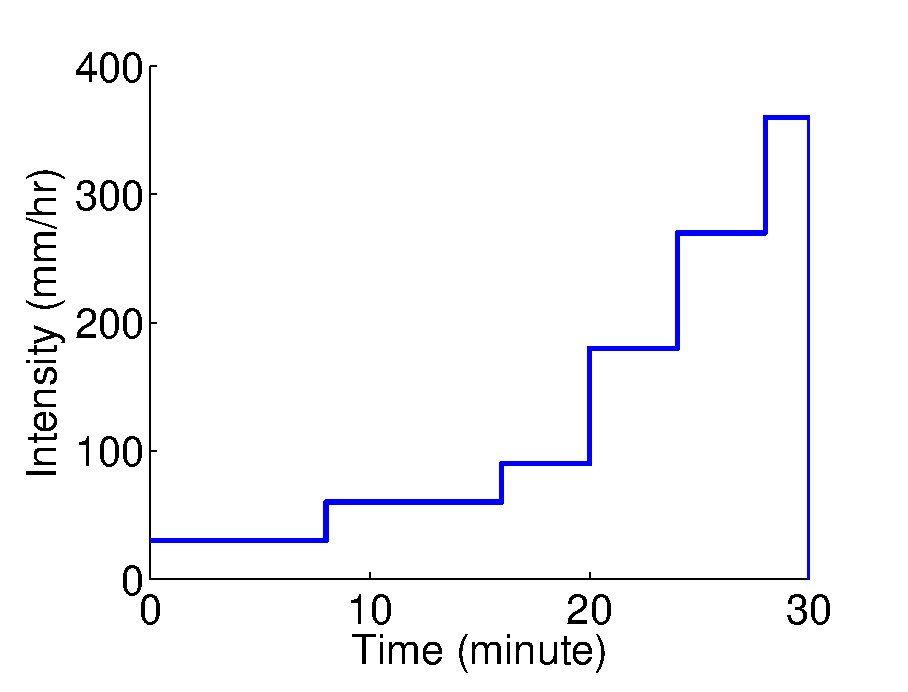
\includegraphics[width=0.24\textwidth]{./img/rg2_input_increase}}
  \subfloat[]{%
  \label{fig:rg2inputdecrease}
  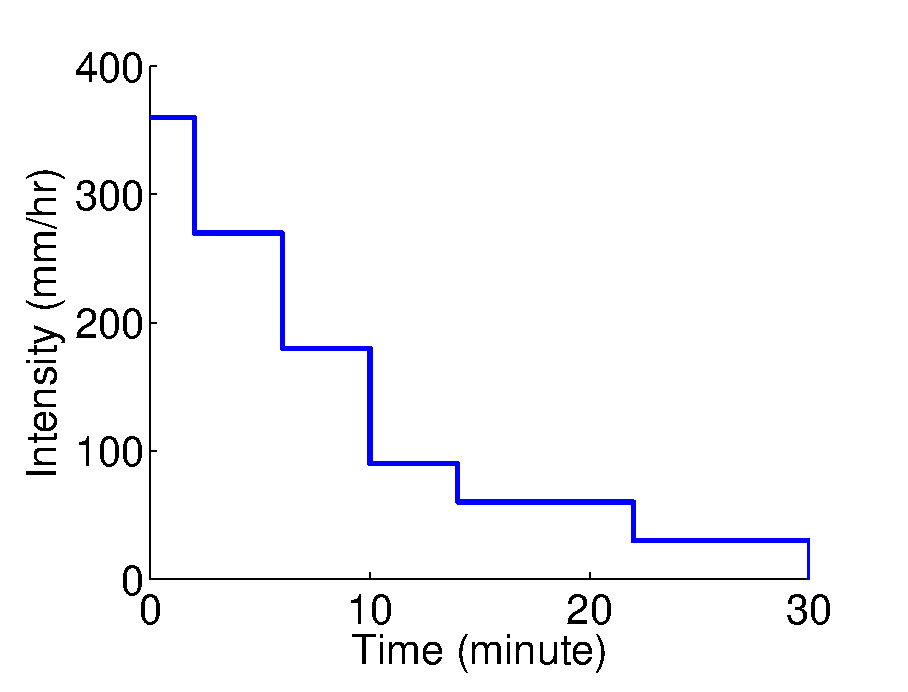
\includegraphics[width=0.24\textwidth]{./img/rg2_input_decrease}}
  \subfloat[]{%
  \label{fig:rg2inputcontrol}
  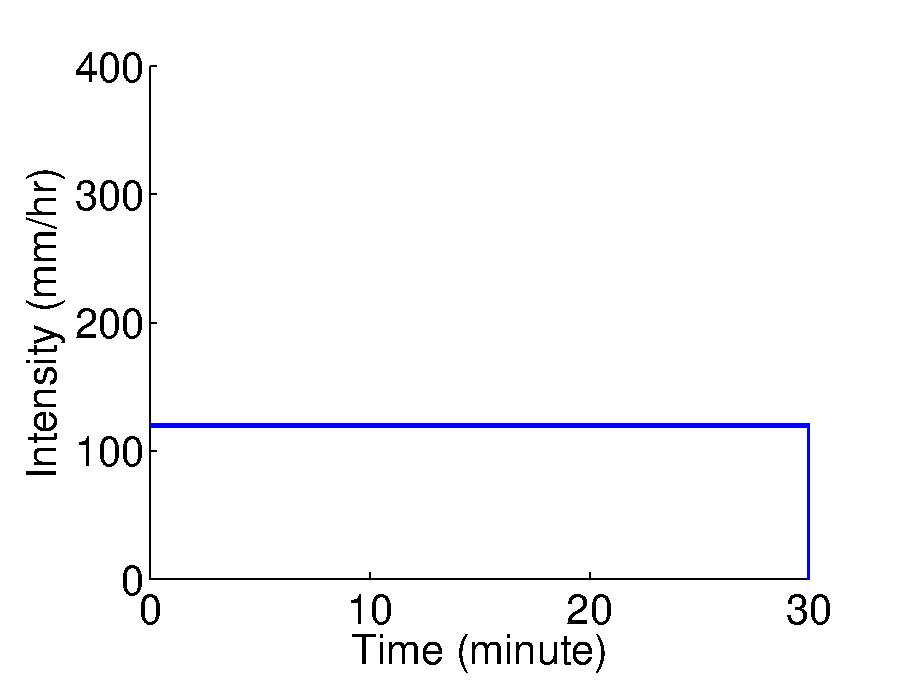
\includegraphics[width=0.24\textwidth]{./img/rg2_input_control}}
  \subfloat[]{%
  \label{fig:rg2inputincreasedecrease}
  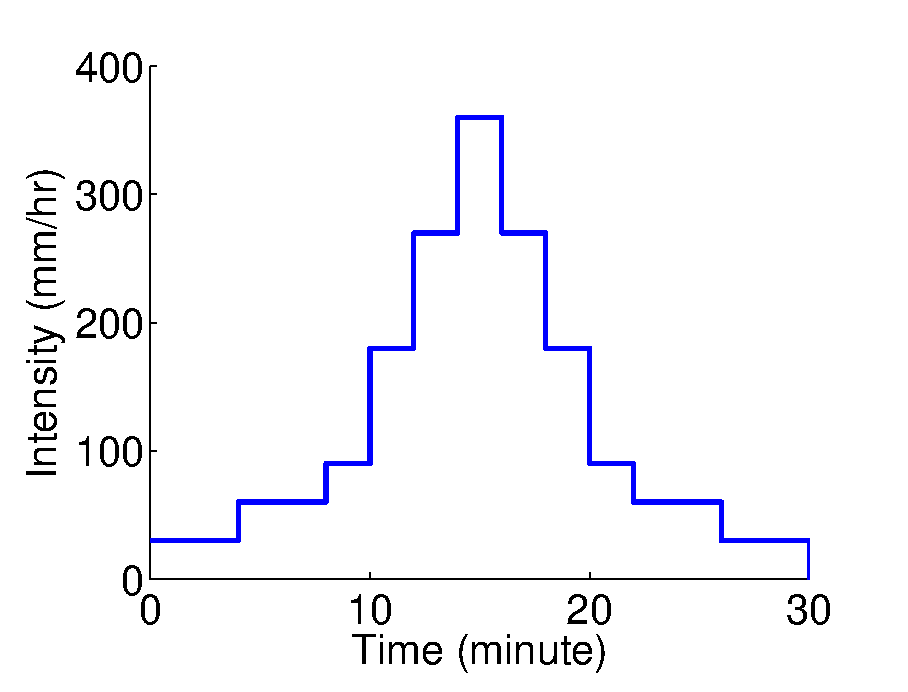
\includegraphics[width=0.24\textwidth]
{./img/rg2_input_increase_decrease}}
  \caption[Intensity input patterns for RillGrow2 simulations.]{Intensity
input patterns for RillGrow2 simulations. All the inputs have the same total
rainfall amount and duration (i.e.\ 60 mm rainfall for 30 minutes). Note the
scales of the axes.}
  \label{fig:rillgrow2intensityinputs}
\end{figure}

\section{Effects on Runoff and Soil Loss}
\label{sec:ImplicationsOfRainfallIntensityChangesOnRunoffandSoilLoss}

The results of WEPP, EUROSEM and RillGrow simulations are summarised in Table
\ref{tab:WEPPSimulationResults}, Table \ref{tab:EUROSEMimulationResults} and
Table \ref{tab:RillGrowSimulationResults}.

\begin{table}[htbp]
  \figureversion{tabular}
  \caption{WEPP simulation results}
  \label{tab:WEPPSimulationResults}
  \centering
    \begin{tabular}{lcccc}
      \toprule
      Storm Pattern & \multicolumn{2}{c}{\textbf{60 mm/hr}} &
\multicolumn{2}{c}{\textbf{10 mm/hr}}\\
      \cmidrule(r){2-3} \cmidrule(l){4-5}
      & runoff  & soil loss  & runoff & soil loss\\
      & (mm) & (t/ha) & (mm) & (t/ha)\\
      \midrule
      Constant & 104.2 & 105 & 68.9 & 0.4\\
      Increasing & 104.2 & 114.6 ($+$9.1) & 70.3 ($+$2.0) & 21.4 ($+$5250)\\
      Decreasing & 104.2 & 110.4 ($+$5.1) & 68.6 ($-$0.4) & 15.4 ($+$3750)\\
      Increasing-decreasing & 104.2 & 114.7 ($+$9.2) & 69.9 ($+$1.5) & 22.8
($+$5600)\\
      \bottomrule
      %\addlinespace[1mm]
      \multicolumn{5}{p{10cm}}{\footnotesize Figures in (\ )
are the \% changes from the result with a constant intensity storm. $+/-$
indicates a increase or decrease.}\\
    \end{tabular}
\end{table}

% \begin{sidewaystable}[htbp]
%   \figureversion{tabular}
%   \caption{WEPP simulation results}
%   \label{tab:WEPPSimulationResults}
%   \centering
%     \begin{tabular}{lcccccc}
%       \toprule
%       Storm Pattern & \multicolumn{2}{c}{\textbf{60 mm/hr}} &
% \multicolumn{2}{c}{\textbf{10 mm/hr}} & \multicolumn{2}{c}{\textbf{Mean}}\\
%       \cmidrule(r){2-3} \cmidrule(l){4-5} \cmidrule(l){6-7}
%       & runoff  & soil loss  & runoff & soil loss & runoff &
% soil loss \\
%       & (mm) & (t/ha) & (mm) & (t/ha)& (mm) & (t/ha) \\
%       \midrule
%       Constant & 104.2 & 105 & 68.9 & 0.4 & 86.6 & 52.7 \\
%       Increasing & 104.2 & 114.6 ($+$9.1) & 70.3 ($+$2.0) &
% 21.4 ($+$5250) & 87.3 ($+$0.8) & 68 ($+$29)\\
%       Decreasing & 104.2 & 110.4 ($+$5.1) & 68.6 ($-$0.4)&
% 15.4 ($+$3750) & 86.4 ($-$0.2) & 62.9 ($+$19.4)\\
%       Increasing-decreasing & 104.2 & 114.7 ($+$9.2) & 69.9
% ($+$1.5) & 22.8 ($+$5600) & 87.1 ($+$0.6) & 68.8 ($+$30.6)\\
%       \bottomrule
%       %\addlinespace[1mm]
%       \multicolumn{7}{p{15cm}}{\footnotesize Figures in (\ )
% are the \% changes from the result with a constant intensity storm. $+/-$
% indicates a increase or decrease.}\\
%     \end{tabular}
% \end{sidewaystable}

\begin{table}[htbp]
  \figureversion{tabular}
  \caption{EUROSEM simulation results}
  \label{tab:EUROSEMimulationResults}
  \centering
    \begin{tabular}{lcccc}
      \toprule
      Storm Pattern & \multicolumn{2}{c}{\textbf{60 mm/hr}} &
\multicolumn{2}{c}{\textbf{10 mm/hr}}\\
      \cmidrule(r){2-3} \cmidrule(l){4-5}
      & runoff  & soil loss  & runoff & soil loss \\
      & (mm) & (t/ha) & (mm) & (t/ha) \\
      \midrule
      Constant   & 101.4 & 22.6 & 73.8 & 24.7\\
      Increasing & 98.7 ($-$2.7)& 19.7 ($-$12.8)& 75.5 ($+$2.3)& 22.1
($-$10.5)\\
      Decreasing & 103.5 ($+$2.1)& 22.2 ($-$1.8)& 74.0 ($+$0.3) & 24.1
($-$2.4)\\
      Increasing-decreasing & 103.3 ($+$1.9)& 21.0 ($-$7.1)& 76.0 ($+$3.0)& 22.7
($-$8.1)\\
      \bottomrule
      %\addlinespace[1mm]
      \multicolumn{5}{p{10cm}}{\footnotesize Figures in (\ )
are the \% changes from the result with a constant intensity storm. $+/-$
indicates a increase or decrease.}\\
    \end{tabular}
\end{table}

% \begin{sidewaystable}[htbp]
%   \figureversion{tabular}
%   \caption{EUROSEM simulation results}
%   \label{tab:EUROSEMimulationResults}
%   \centering
%     \begin{tabular}{lcccccc}
%       \toprule
%       Storm Pattern & \multicolumn{2}{c}{\textbf{60 mm/hr}} &
% \multicolumn{2}{c}{\textbf{10 mm/hr}} & \multicolumn{2}{c}{\textbf{Mean}}\\
%       \cmidrule(r){2-3} \cmidrule(l){4-5} \cmidrule(l){6-7}
%       & runoff  & soil loss  & runoff & soil loss & runoff &
% soil loss \\
%       & (mm) & (t/ha) & (mm) & (t/ha)& (mm) & (t/ha) \\
%       \midrule
%       Constant   & 101.4 & 22.6 & 73.8 & 24.7 & 87.6 & 23.7 \\
%       Increasing & 98.7 ($-$2.7)& 19.7 ($-$12.8)& 75.5
% ($+$2.3)& 22.1 ($-$10.5)& 87.1 ($-$0.6)& 21.0 ($-$11.4)\\
%       Decreasing & 103.5 ($+$2.1)& 22.2 ($-$1.8)& 74.0 ($+$0.3) & 24.1 ($-$2.4)&
% 88.8 ($+$1.4)& 23.2 ($-$2.1)\\
%       Increasing-decreasing & 103.3 ($+$1.9)& 21.0 ($-$7.1)&
% 76.0 ($+$3.0)& 22.7 ($-$8.1)& 89.7 ($+$2.4)& 21.9 ($-$7.6)\\
%       \bottomrule
%       %\addlinespace[1mm]
%       \multicolumn{7}{p{15cm}}{\footnotesize Figures in (\ )
% are the \% changes from the result with a constant intensity storm. $+/-$
% indicates a increase or decrease.}\\
%     \end{tabular}
% \end{sidewaystable}

\begin{table}[htbp]
  \figureversion{tabular}
  \centering
  \small
  \caption{RillGrow simulation results}
  \label{tab:RillGrowSimulationResults}
    \begin{tabular}{lcc}
    \toprule
     & Totals lost from edges$^\dagger$ (litre) & Soil Loss (t/ha)\\
    \midrule%
    Constant & 471.9 & 64.0 \\
    Increasing & 472.4 ($+$0.1)& 73.5 ($+$14.8)\\
    Decreasing & 471.2 ($-$0.2)& 90.5 ($+$41.4)\\
    Increasing-decreasing & 472.2 ($+$0.1)& 82.6 ($+$29.1)\\
    \bottomrule
    %\addlinespace[1mm]
    \multicolumn{3}{p{11cm}}{\footnotesize $^\dagger$ No
infiltration was considered. Every rain runs off the edge of the simulated plot.
Figures in (\ ) are the \% changes from the result with a constant intensity
storm. $+/-$ indicates a increase or decrease.}\\
    \end{tabular}
\end{table}

\section{Discussion}
\label{sec:ImpactsOfRainfallIntensityChangesOnRunoffAndErosionDiscussion}

In WEPP, WSIP is parameterized as $t_p$ which represents normalised
time-to-peak. This value was considered not much sensitive previously
\citep{nearing1990-839}.

%Discuss how the models respond to each rainfall patterns. Which one
%produced most runoff and soil loss?
%Which on produced least runoff and soil loss?

%What's the potential problem with constant intensity generating least
%runoff and soil loss (WEPP)?
%GCM and RCM data scale. knowing average daily rainfall intensity is not
%sufficient for erosion estimation. It may lead to underestimated erosion
%with low average intensity rainfall.

In this investigation, it is clear that WSIP is important for soil erosion
estimation. Without knowing future WSIPs, it could easily lead to erroneous
results. Moreover, when average rainfall intensity (i.e.\ constant rainfall
intensity) of low intensity events are used for erosion modelling, WEPP
immensely underestimates soil loss rates by about 50 times less than average
soil loss of other WISPs. This is a considerable
difference in comparison to runoff values which are similar for all four
cases (Table \ref{tab:WEPPSimulationResults}). This result with constant
intensity is consistent with \citet{parsons2006-68}.

\citet{parsons2006-68} conducted a lab test to investigate the effects of
intra-storm patterns (WSIPs) on soil erosion. They found that the
constant-intensity storm generated about 75\% of the average soil loss for the
variable-intensity storms.

\begin{table}[htbp]
  \figureversion{tabular}
  \caption[Experiment results]{Experiment results
\citep[From][]{parsons2006-68}}
  \label{tab:Tonysexperimentresults}
  \scriptsize
  \centering
    \begin{tabular}{lcccccccccc}
      \toprule
      Storm Pattern & \multicolumn{2}{c}{Clay loam} &
\multicolumn{2}{c}{\textbf{Sandy loam}} & \multicolumn{2}{c}{Sandy soil} &
\multicolumn{2}{c}{\textbf{Total}}\\
      \cmidrule(r){2-3} \cmidrule(rl){4-5} \cmidrule(rl){6-7}
\cmidrule(l){8-9}
      & runoff (l) & loss (g) & runoff (l) & loss (g) & runoff
(l) & loss (g) & runoff (l) & loss (g)\\
      \midrule
      Constant & 131.6 & 523 & 83.4  & 1256 & 110.2 & 2509 &
325.2 & 4289\\
      Increasing & 108.2 & 748 & 93.0  & 2435 & 72.2 & 1947 &
273.4 & 5130 \\
      Decreasing & 101.3 & 456 & 114.0 & 3230 & 108.3 & 2862 &
323.6 & 6548 \\
      Rising-falling & 110.4 & 631 & 95.8  & 2110 & 114.2 &
3584 & 320.4 & 6324\\
      Falling-rising$^\dagger$ & 103.6 & 629 & 103.9  & 1645 &
108.1 & 3275 & 315.6 & 5549\\
      \bottomrule
      %\addlinespace[1mm]
      \multicolumn{9}{p{11cm}}{\footnotesize $^\dagger$ Not
used in this research since only one peak intensity is assumed for all model
simulations.}\\
    \end{tabular}
\end{table}

RillGrow estimated the similar effects on soil loss as the result of
\citet{parsons2006-68}. RillGrow simulated, for constant intensity rainfall,
about 78\% soil loss from the average soil loss of other storms. It also
estimated more soil loss for the storm with decreasing intensity than other
storm patterns.

WEPP, EUROSEM and RillGrow results with varying WSIPs are
compared with the result from \citet{parsons2006-68} in Table
\ref{tab:MagnitudeofSoilLossAffectedByIntraStormPatterns}.

\begin{table}[htbp]
  \centering
  \scriptsize
  \caption{Magnitude of soil loss affected by WSIPs}
  \label{tab:MagnitudeofSoilLossAffectedByIntraStormPatterns}
    \begin{tabular}{cllll}
      \toprule
      Soil Loss & \citet{parsons2006-68}  & WEPP & EUROSEM &
RillGrow \\
                & (Sandy loam) & (Mean) & (Mean) & \\
      \midrule
      High & decreasing & increasing-decreasing & constant &
decreasing\\
      $\Uparrow$ & increasing & increasing & decreasing &
increasing-decreasing\\
      $\Downarrow$ & increasing-decreasing & decreasing &
increasing-decreasing & increasing\\
      Low & constant & constant & increasing & constant\\
      \bottomrule
    \end{tabular}
\end{table}


%\begin{enumerate}
% \item What information do we need about rainfall intensity for soil
%erosion estimation?
% \item Desirability of different ways of expressing future rainfall
%intensity
% \begin{enumerate}
%   \item TP \& IP
%   \item Breakpoint data without no rainfall periods
%   \item Breakpoint data with no rainfall periods
%   \item Event rainfall data (i.e., tipping bucket data)
% \end{enumerate}
% \item What kind of data format do we need? Breakpoint with no rain
%periods (NRPs), Breakpoint without NRPs or TP/IP?
% \item Effect of timing of peak intensity
% \begin{enumerate}
%   \item Choose seasonal events (Jan, Apr, Jul and Oct)
%   \item Calibrate initial conditions for the events according to
%season $\rightarrow$ No need! See the initial condition note.
%   \item Run WEPP with TP/IP method $\rightarrow$ these output
%could be used as control
%   \item modify peak intensity time to 0.01, 0.25, 0.5, 0.75, 0.99
%and 1 (for constant intensity)
% \end{enumerate}
% \item We need to have sub-daily data for soil erosion estimation. Then,
%how much short is short enough for temporal resolution of rainfall data for
%soil erosion estimation? 1-min -- 12 hrs?
%\end{enumerate}

%xie2002-1843? may be useful for discussion?

When WEPP,for example, is to be used for erosion estimations, it is
necessary to know $t_p$ and $i_p$ values of the rainfall storm for the
simulation.
As can be seen in Table \ref{tab:WEPPSimulationResults}, the presence of
$t_p$ have some effects on the result of simulations. It becomes more
evident when rainfall with low intensity is considered.

\citet{nearing1990-839} performed sensitivity analysis on WEPP, which was
still in the process of development, by assessing various input variables
such as soil, plant residue and canopy, hillslope topography, and hydrologic
input variables. They calculated sensitivity parameter, S, as a relative
normalised change in output to a normalised change in input.
They concluded that peak rainfall intensity, time to peak rainfall
intensity, rill spacing and width, and sediment transportability were not
playing a major role in soil loss predictions.

Because of the fact that their analysis was carried out on the developing
version of WEPP and this chapter used the new version of WEPP, their
findings may not be compared directly with the result presented in this
chapter. However, it is interesting to note that they used relatively high
rainfall intensity as a base value for the single storm model input
parameter. They used 100 mm/hr intensity while 10 and 60 mm/hr were used for
the analysis carried out in this chapter.
%This allows direct comparisons of sensitivities for input parameters which
%have different orders of magnitude.

%This echoes the findings by \citet{nearing1990-839}. need to cross check
%with Nearing1990. look for what intensity did he use for the storm. eg. is
%it close to 10 or 60 mm/hr?

However, when there is no peak intensity, in other words, when intensity is
constant, considerably less soil loss was generated in comparison to the
ones with a intensity peak.
This shows a problem in using RCM rainfall data directly for soil erosion
modelling because they usually comes as daily data.

\section{Conclusion}
\label{sec:ImpactsOfRainfallIntensityChangesOnRunoffAndErosionConclusion}
WSIP affects the soil erosion amount.
Runoff does not seem to be affected by WSIP
changes.
WSIP of events with high intensity have less
influence on erosion rate. Events with a constant low intensity produced
dramatically less erosion. This results is consistent with the lab
experiment and modelling.

%\chapter{SUMMARY OF MODEL SIMULATION RESULTS}
%\label{sec:SUMMARYANDLIMITATIONSOFEROSIONMODELS}





%\section{Limitations of Erosion Models}
%\label{sec:LimitationsOfErosionModels}



%Although erosion models used in this research requires high resolution
%rainfall data, such kind of data is not readily available, and seldom is
%complete and long term. This is because it is usually aggregated into other
%scales for ease of storage and portability.

%Suggestions on possible improvements of WEPP and EUROSEM for rainfall
%intensity

%Discussion about the assumption of daily rainfall = single storm---pros \&
%cons for future soil erosion estimation.

%$\filledstar\filledstar\filledstar$ Unmatched disaggregated rainfall data
%by WEPP:
%
%WEPP is doing something weird.
% When time intervals shorter than an hour were used for WEPP simulations,
% WEPP reconstructs breakpoint data from original breakpoint data to ``WEPP
% interpreted'' breakpoint data, which has different intensity information.
% The total number of breakpoint are the same so as the accumulated amount.
% However, because the time increments are changed by WEPP, rainfall intensity
% information for the original breakpoint data is not the same.
% This means that:
% \begin{enumerate}
%   \item Resulting runoff and soil loss may be estimated unrealistically,
% considering rainfall intensity is different from the observation;
%   \item Studies on impacts of rainfall intensity change on soil erosion with
% rainfall data shorter than hourly may result in runoff and soil loss
% estimations which is different from original rainfall intensity.
% \end{enumerate}
% Using breakpoint data shorter than hourly will result in feeding in wrong
% rainfall intensity information to WEPP.
% This problem seems important because it will consequently alter the original
% rainfall intensity even if we use breakpoint data in order to keep the
% original rainfall intensity unchanged. This is because breakpoint rainfall
% data are better representations of the real rainfall intensity than CLIGEN
% rainfall data (See Chapter \ref{sec:EFFECTSOFTEMPORALSCALESOFSTROMDATA})

WEPP usually requires four stages of rainfall data conversion in order to
simulate runoff and soil loss:
\begin{enumerate*}
  \item Starting with the original time step rainfall data
  \item Converting to an aggregated time stepped rainfall data by removing no
rainfall periods
  \item Parametrising the rainfall data into amount, duration, time to peak and
peak intensity
  \item Finally, regenerating disaggregated rainfall data based on the
parameters
\end{enumerate*}

After each stage, original rainfall intensity information is lost and distorted
as this research has shown.

WEPP and EUROSEM do not consider temporal variations in erodibility during a
rainfall storm. \citet{kinnell2005-2815} also pointed out this problem with WEPP
and EUROSEM. In the case of raindrop-impact-induced erosion, current so-called
process-based erosion models appear to represent the process involved
inadequately in some respects because the process involved in detachment and
transport of soil from the surface during experiments leading to model
parametrization is unknown \citep{kinnell2005-2815}.

%\citet{Parsons2006-68} found that the constant-intensity storm caused 75\%
%less erosion than the average value for the variable-intensity storms.
%
%``The assumption that a given rainfall intensity falling on a given soil
%for a given amount of time will result in a given amount of runoff and
%erosion is unsound.'' \citep{Parsons2006-68}
%
%``\ldots failing to take account of the context within which a particular
%rainfall intensity occurs and that parametrising equations using
%constant-intensity rainstorms may lead to errors in the prediction of
%interrill soil erosion.'' \citep{Parsons2006-68}
%
%``Models (USLE and WEPP) that derive interrill soil erosion directly from
%rainfall intensity can be expected to perform poorly in predicting soil
%erosion from storms exhibiting temporal variability in rainfall intensity
%as is characteristic of many runoff-producing storm events.''
%\citep{Parsons2006-68}
%
%``Other models (EUROSEM and LISEM) modulate the effect of rainfall
%intensity on erosion by assuming that detachment is controlled both by
%rainfall intensity and runoff depth and that erosion is further controlled
%by interrill transport capacity.'' \citep{Parsons2006-68}
%
%``Neither models that relate interrill soil erosion directly to rainfall
%intensity, nor those that modulate the effect of rainfall intensity by
%runoff depth and transport capacity can account for the observed effects of
%storm pattern on soil erosion.'' \citep{Parsons2006-68}

%In this section, WEPP's possible problem with `re-disaggregation' of
%original breakpoint data that are shorter than hourly should be included.
%
%$\downarrow$ this seems a repeat of what has been said before, but it need
%to be clarified that the second paragraph is true for breakpoint data.
%These problems may only be the cases for CLIGEN-generated data, not
%breakpoint data.
%
%$\filledstar\filledstar\filledstar$ WEPP generally disaggregates CLIGEN
%rainfall data into a form of breakpoint data with 10 breakpoints for
%erosion simulations. This is only true for storms that last over 60-min.
%When a storm lasts less than 60-min, WEPP disaggregates the rainfall data
%into less than ten breakpoints.
%
%$\filledstar\filledstar\filledstar$ This is a problem for BP data of 1-min
%rainfall events that last shorter than 60-min. Even if the 1-min rainfall
%has several breakpoints, it could be represented as, in a worst case, a
%single peak of rainfall which has constant (average) rainfall intensity for
%the storm duration.




%\nolinenumbers

%It seems infiltration rate is responsible for this result.
